\section{子问题三：里程焦虑敏感度识别}

\subsection{问题定义与难点}

任务三聚焦于里程焦虑高敏感用户的识别。按赛题建议，将原始range\_anxiety\_score（1--10分）二值化：评分$>$5为高焦虑（1），$\le$5为低焦虑（0）。样本量基本五五开（低焦虑50.8\% vs 高焦虑49.2\%）。评分权重40\%。

核心难点有三层。第一层，\textbf{标签防泄漏}——标签由range\_anxiety\_score二值化得来，生成后必须把原始评分从特征集里删干净，留一丝都算作弊。第二层，\textbf{边界样本的模糊性}：评分恰好落在5和6的样本，特征分布高度重叠，这恰恰是模型最容易翻车的地方。第三层，\textbf{下游变量风险}——ev\_adoption\_likelihood很可能被里程焦虑直接左右（高焦虑$\to$低采用意愿），主方案不能带这个变量。

\subsection{探索性数据分析}

\subsubsection{目标分布与评分分布}

高低焦虑分类基本均衡（图\ref{fig:t3_target}），无需特别调整类别权重。原始评分分布呈"两端少、中间多"的近似对称形态（图\ref{fig:t3_score}）。有意思的是——阈值恰好切在分布正中心。评分5和6的样本都处在群体密度最高的区间，模型没法靠"记住"某个评分段的特征模式来轻松分类，这本身就是难度所在。

\begin{figure}[H]
\centering
\begin{subfigure}{0.48\textwidth}
\centering
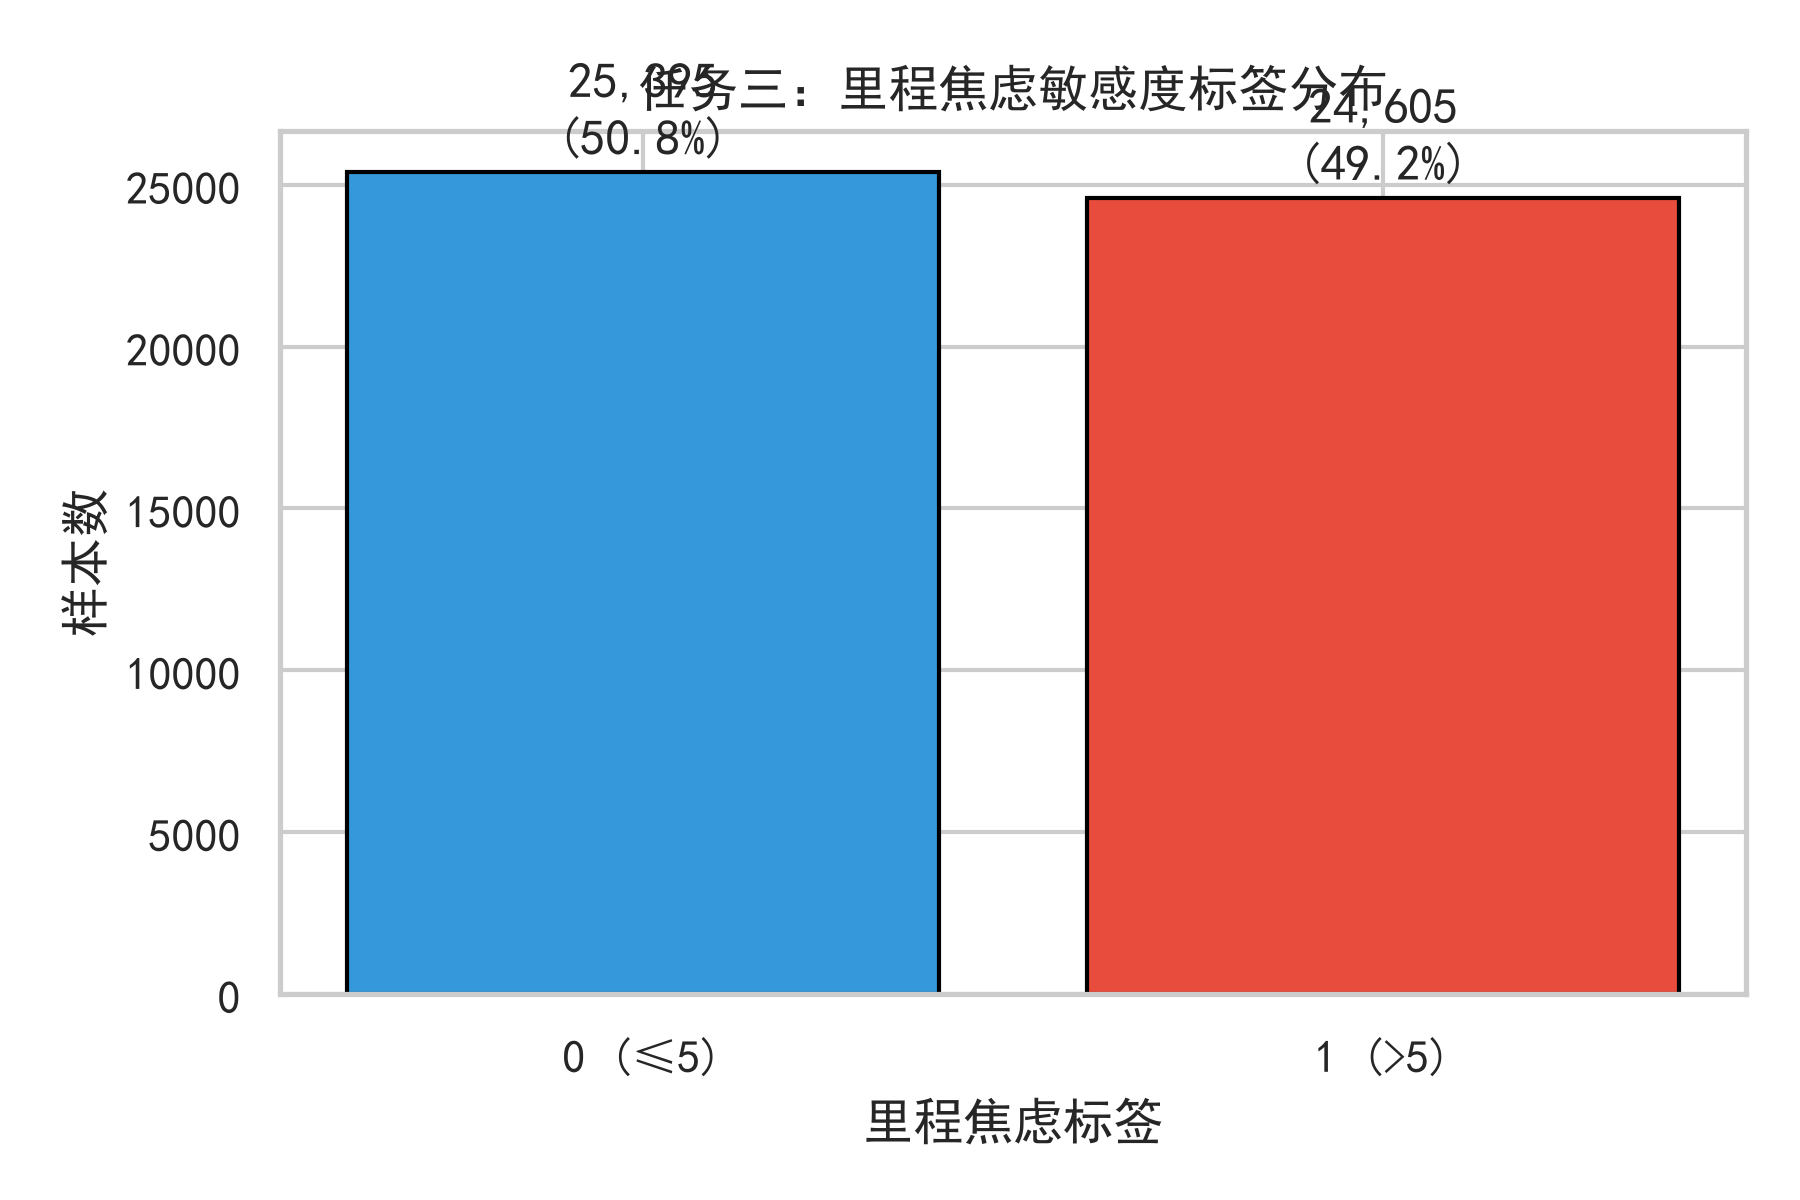
\includegraphics[width=\textwidth]{figures/task3_target_distribution.png}
\caption{目标变量分布}
\label{fig:t3_target}
\end{subfigure}
\hfill
\begin{subfigure}{0.48\textwidth}
\centering
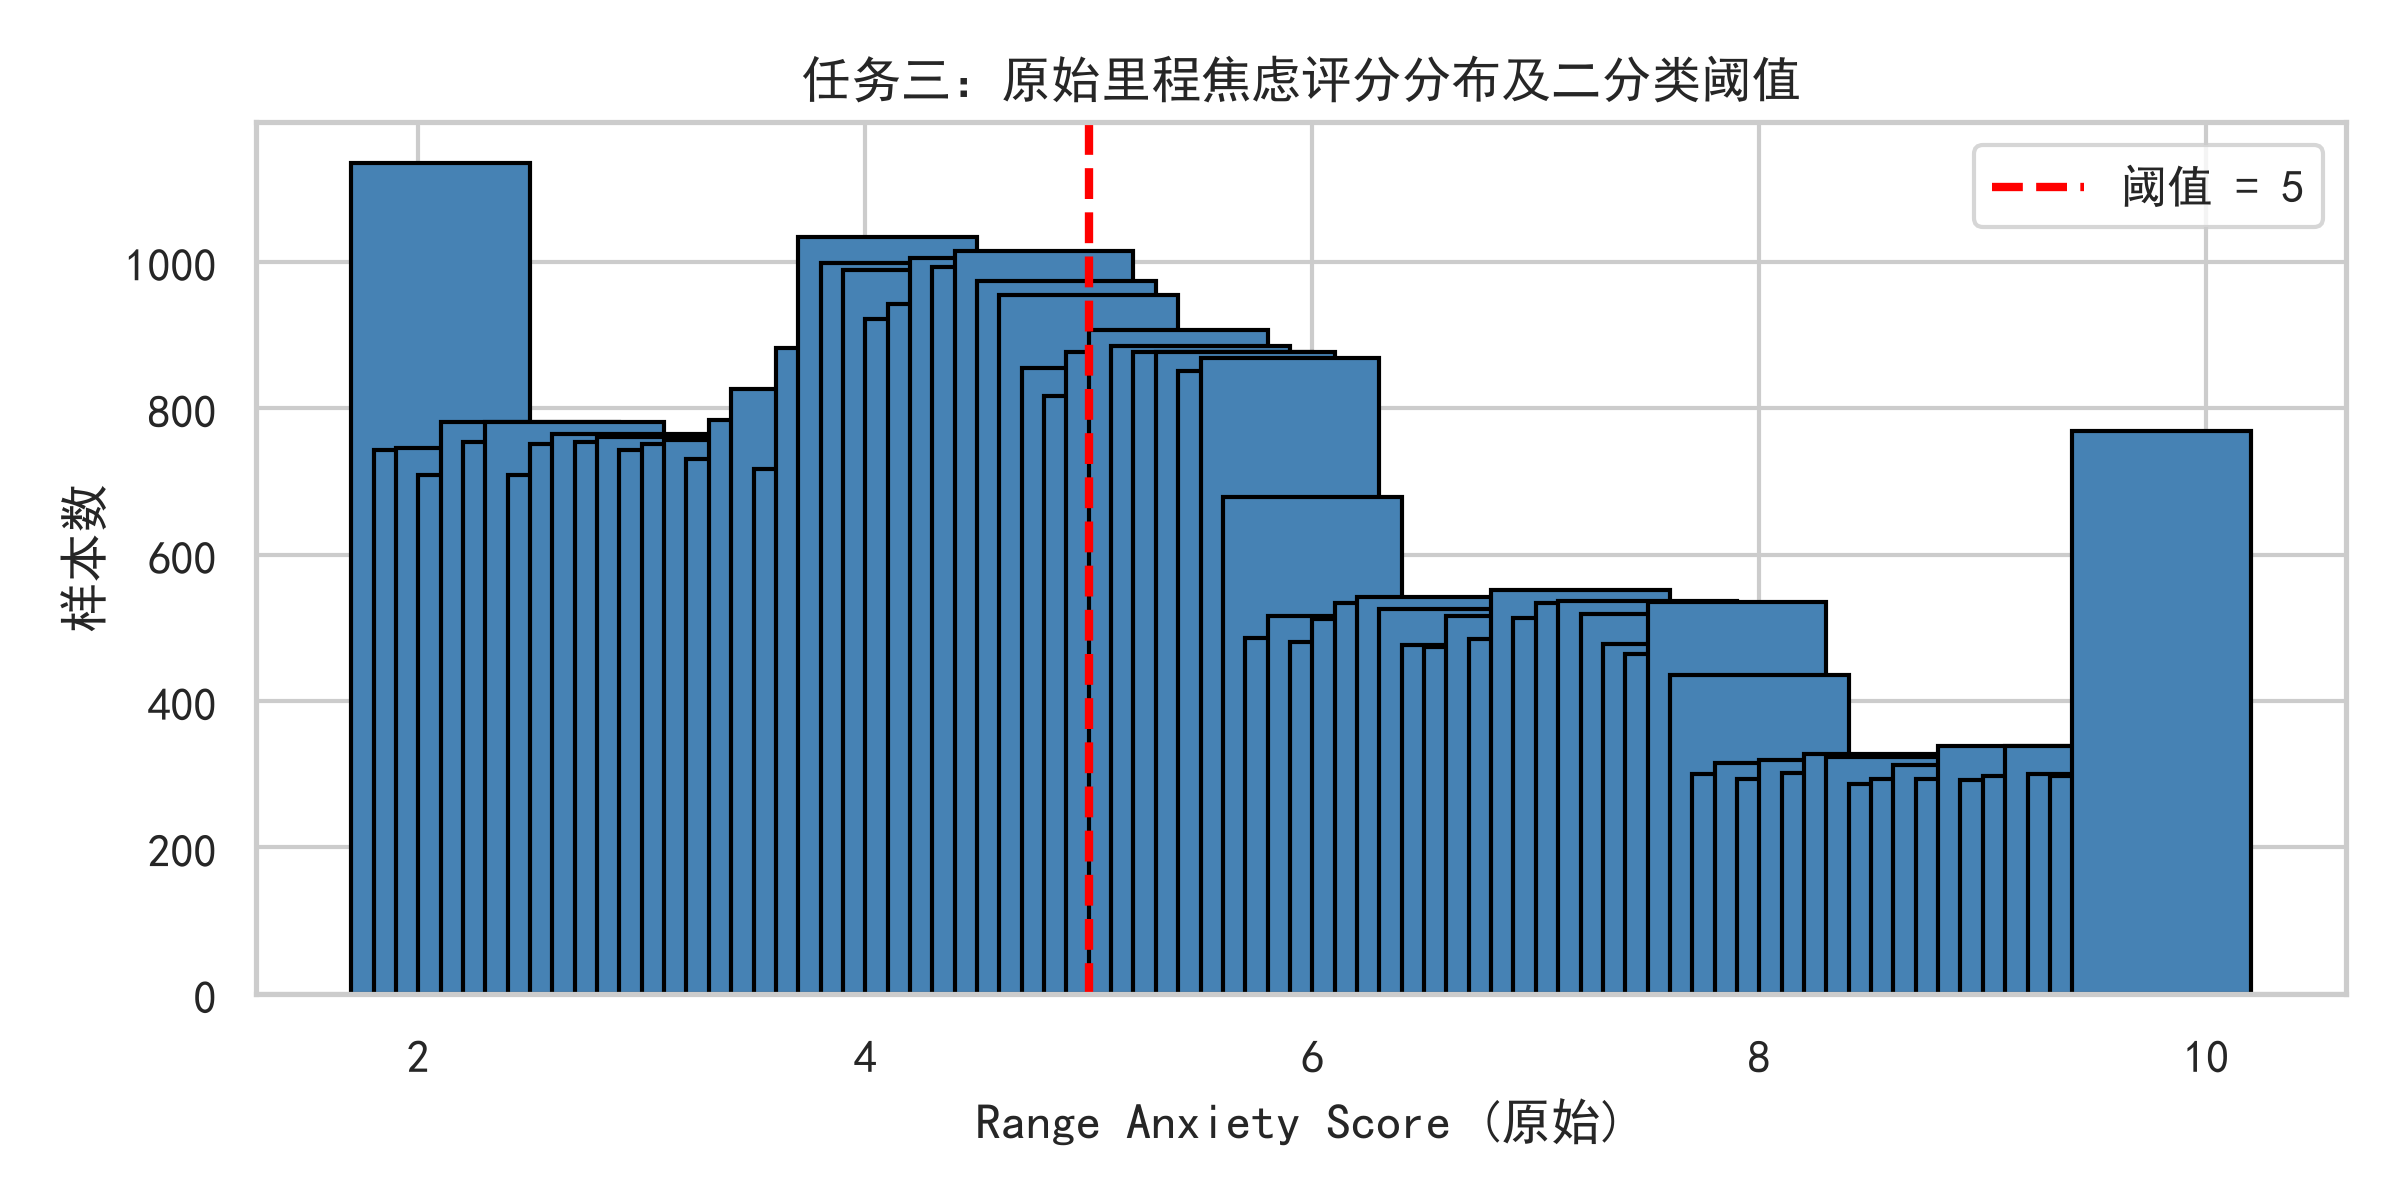
\includegraphics[width=\textwidth]{figures/task3_score_distribution.png}
\caption{原始评分分布及阈值线}
\label{fig:t3_score}
\end{subfigure}
\caption{任务三目标分布与评分分布}
\end{figure}

\subsubsection{充电困难度与EV知识按焦虑分组}

图\ref{fig:t3_box}给出了一条很清晰的趋势。高焦虑组的充电困难度中位数和上四分位数均显著高于低焦虑组；反过来，低焦虑组的EV知识得分中位数明显更高。对电动车技术、成本、充电方式的了解程度，看起来是降低里程焦虑的有效"缓冲"。这个东西可观测，可度量，而且是可干预的——知道得多，焦虑就少。

\begin{figure}[H]
\centering
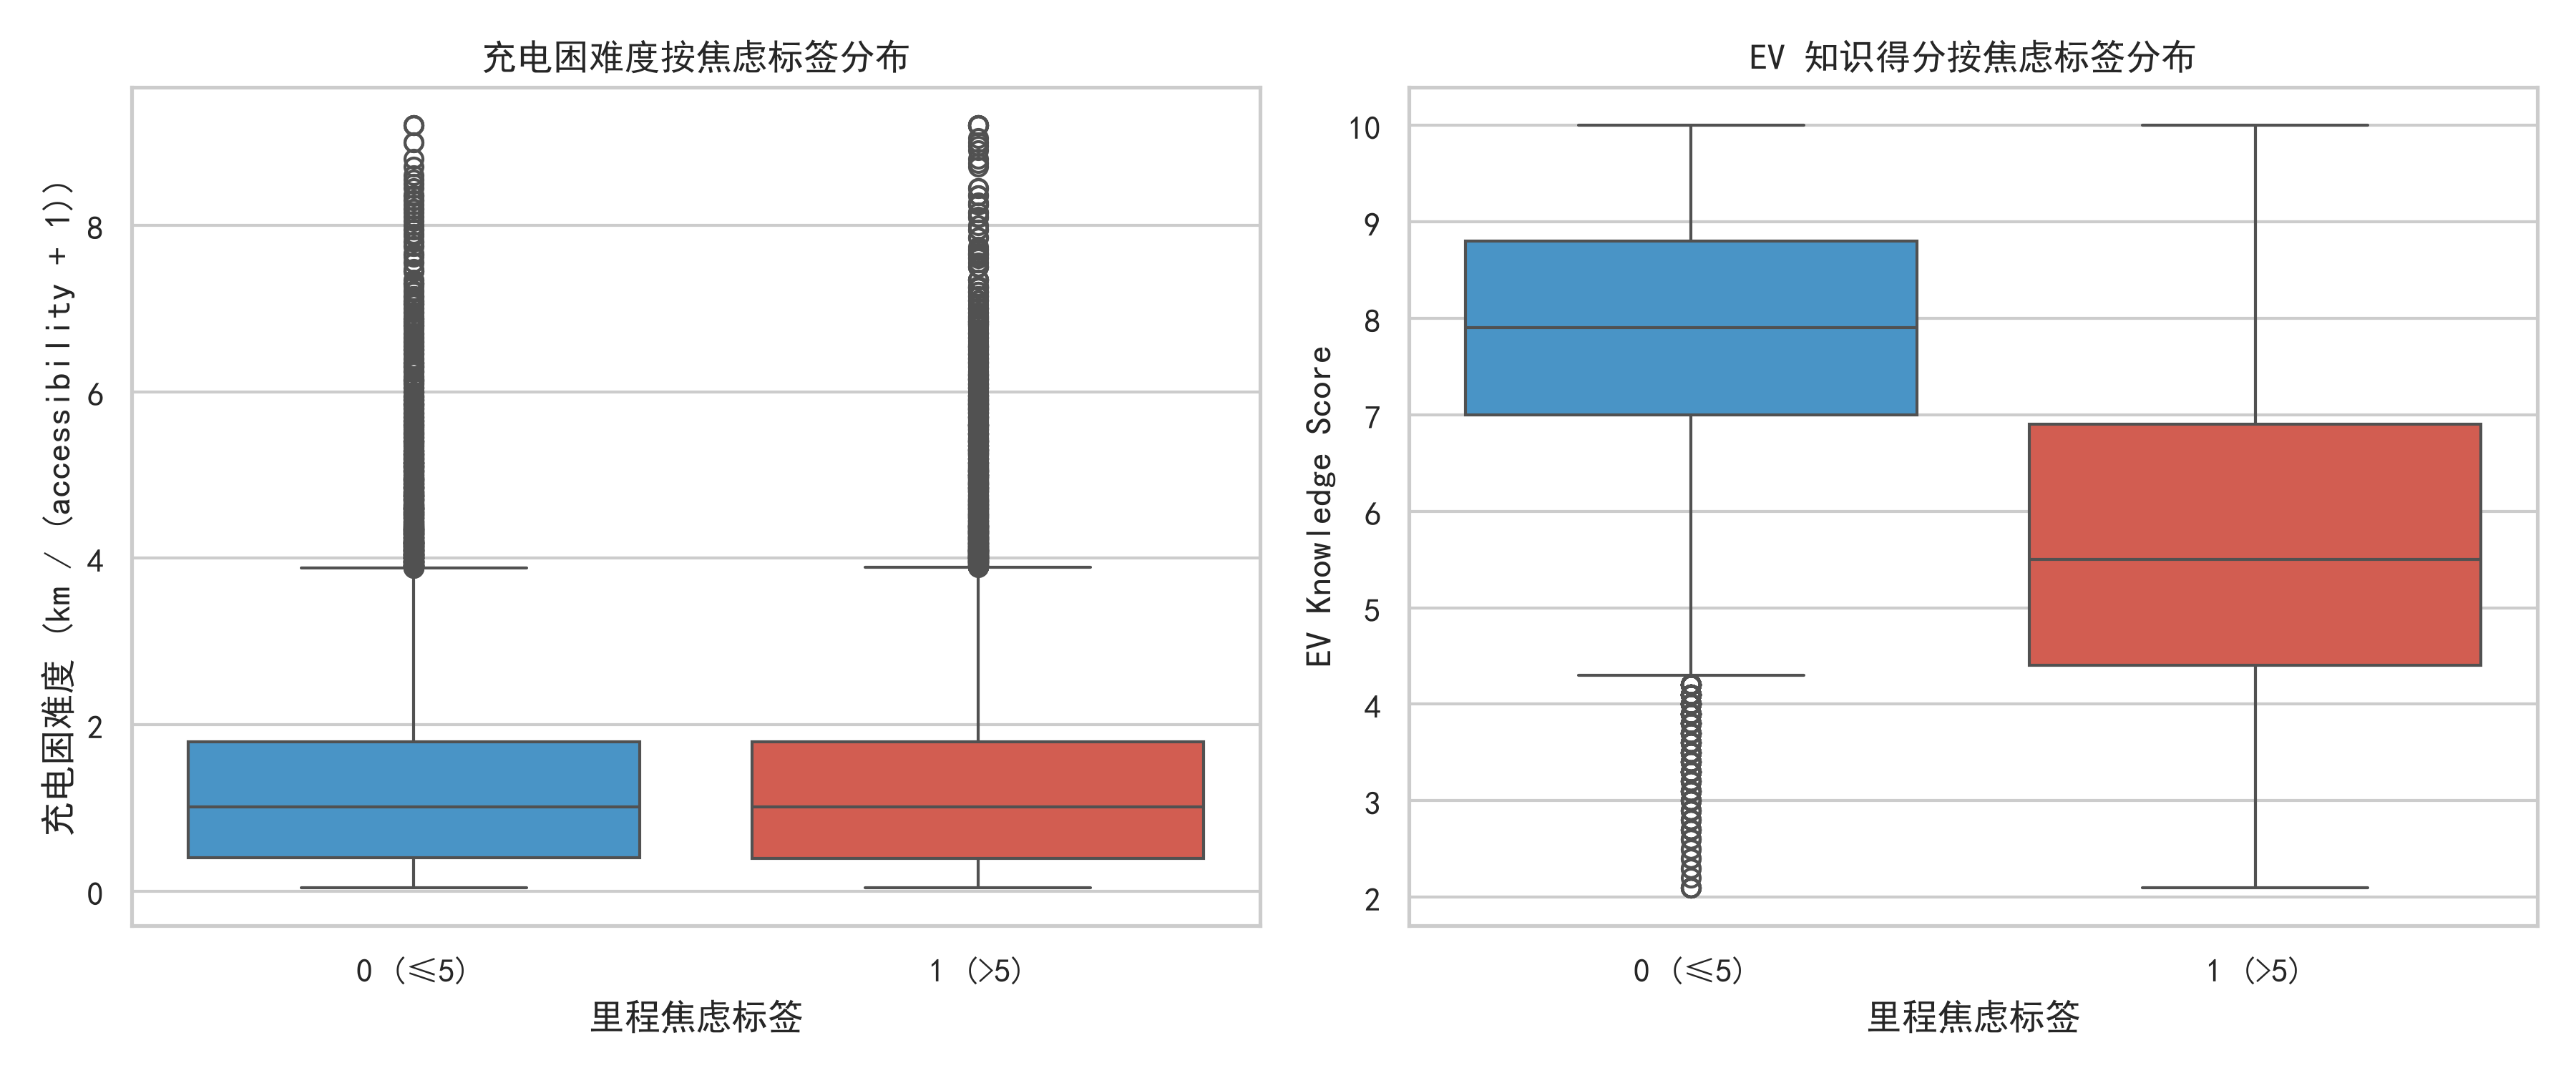
\includegraphics[width=0.8\textwidth]{figures/task3_boxplot_by_target.png}
\caption{充电困难度与EV知识得分按焦虑标签分组箱线图}
\label{fig:t3_box}
\end{figure}

\subsubsection{核心特征相关性}

从热力图（图\ref{fig:t3_corr}）中，我们注意到几条几乎同样强的信号：range\_anxiety\_score与battery\_replacement\_concern呈正相关（+0.63），与technology\_affinity\_score（-0.63）和ev\_knowledge\_score（-0.62）呈负相关。里程焦虑主要由认知/态度维度驱动。相比之下，硬件条件（家充、充电站距离）的单变量区分度低得多——home\_charging\_available与焦虑标签的相关系数仅为-0.012。

\begin{figure}[H]
\centering
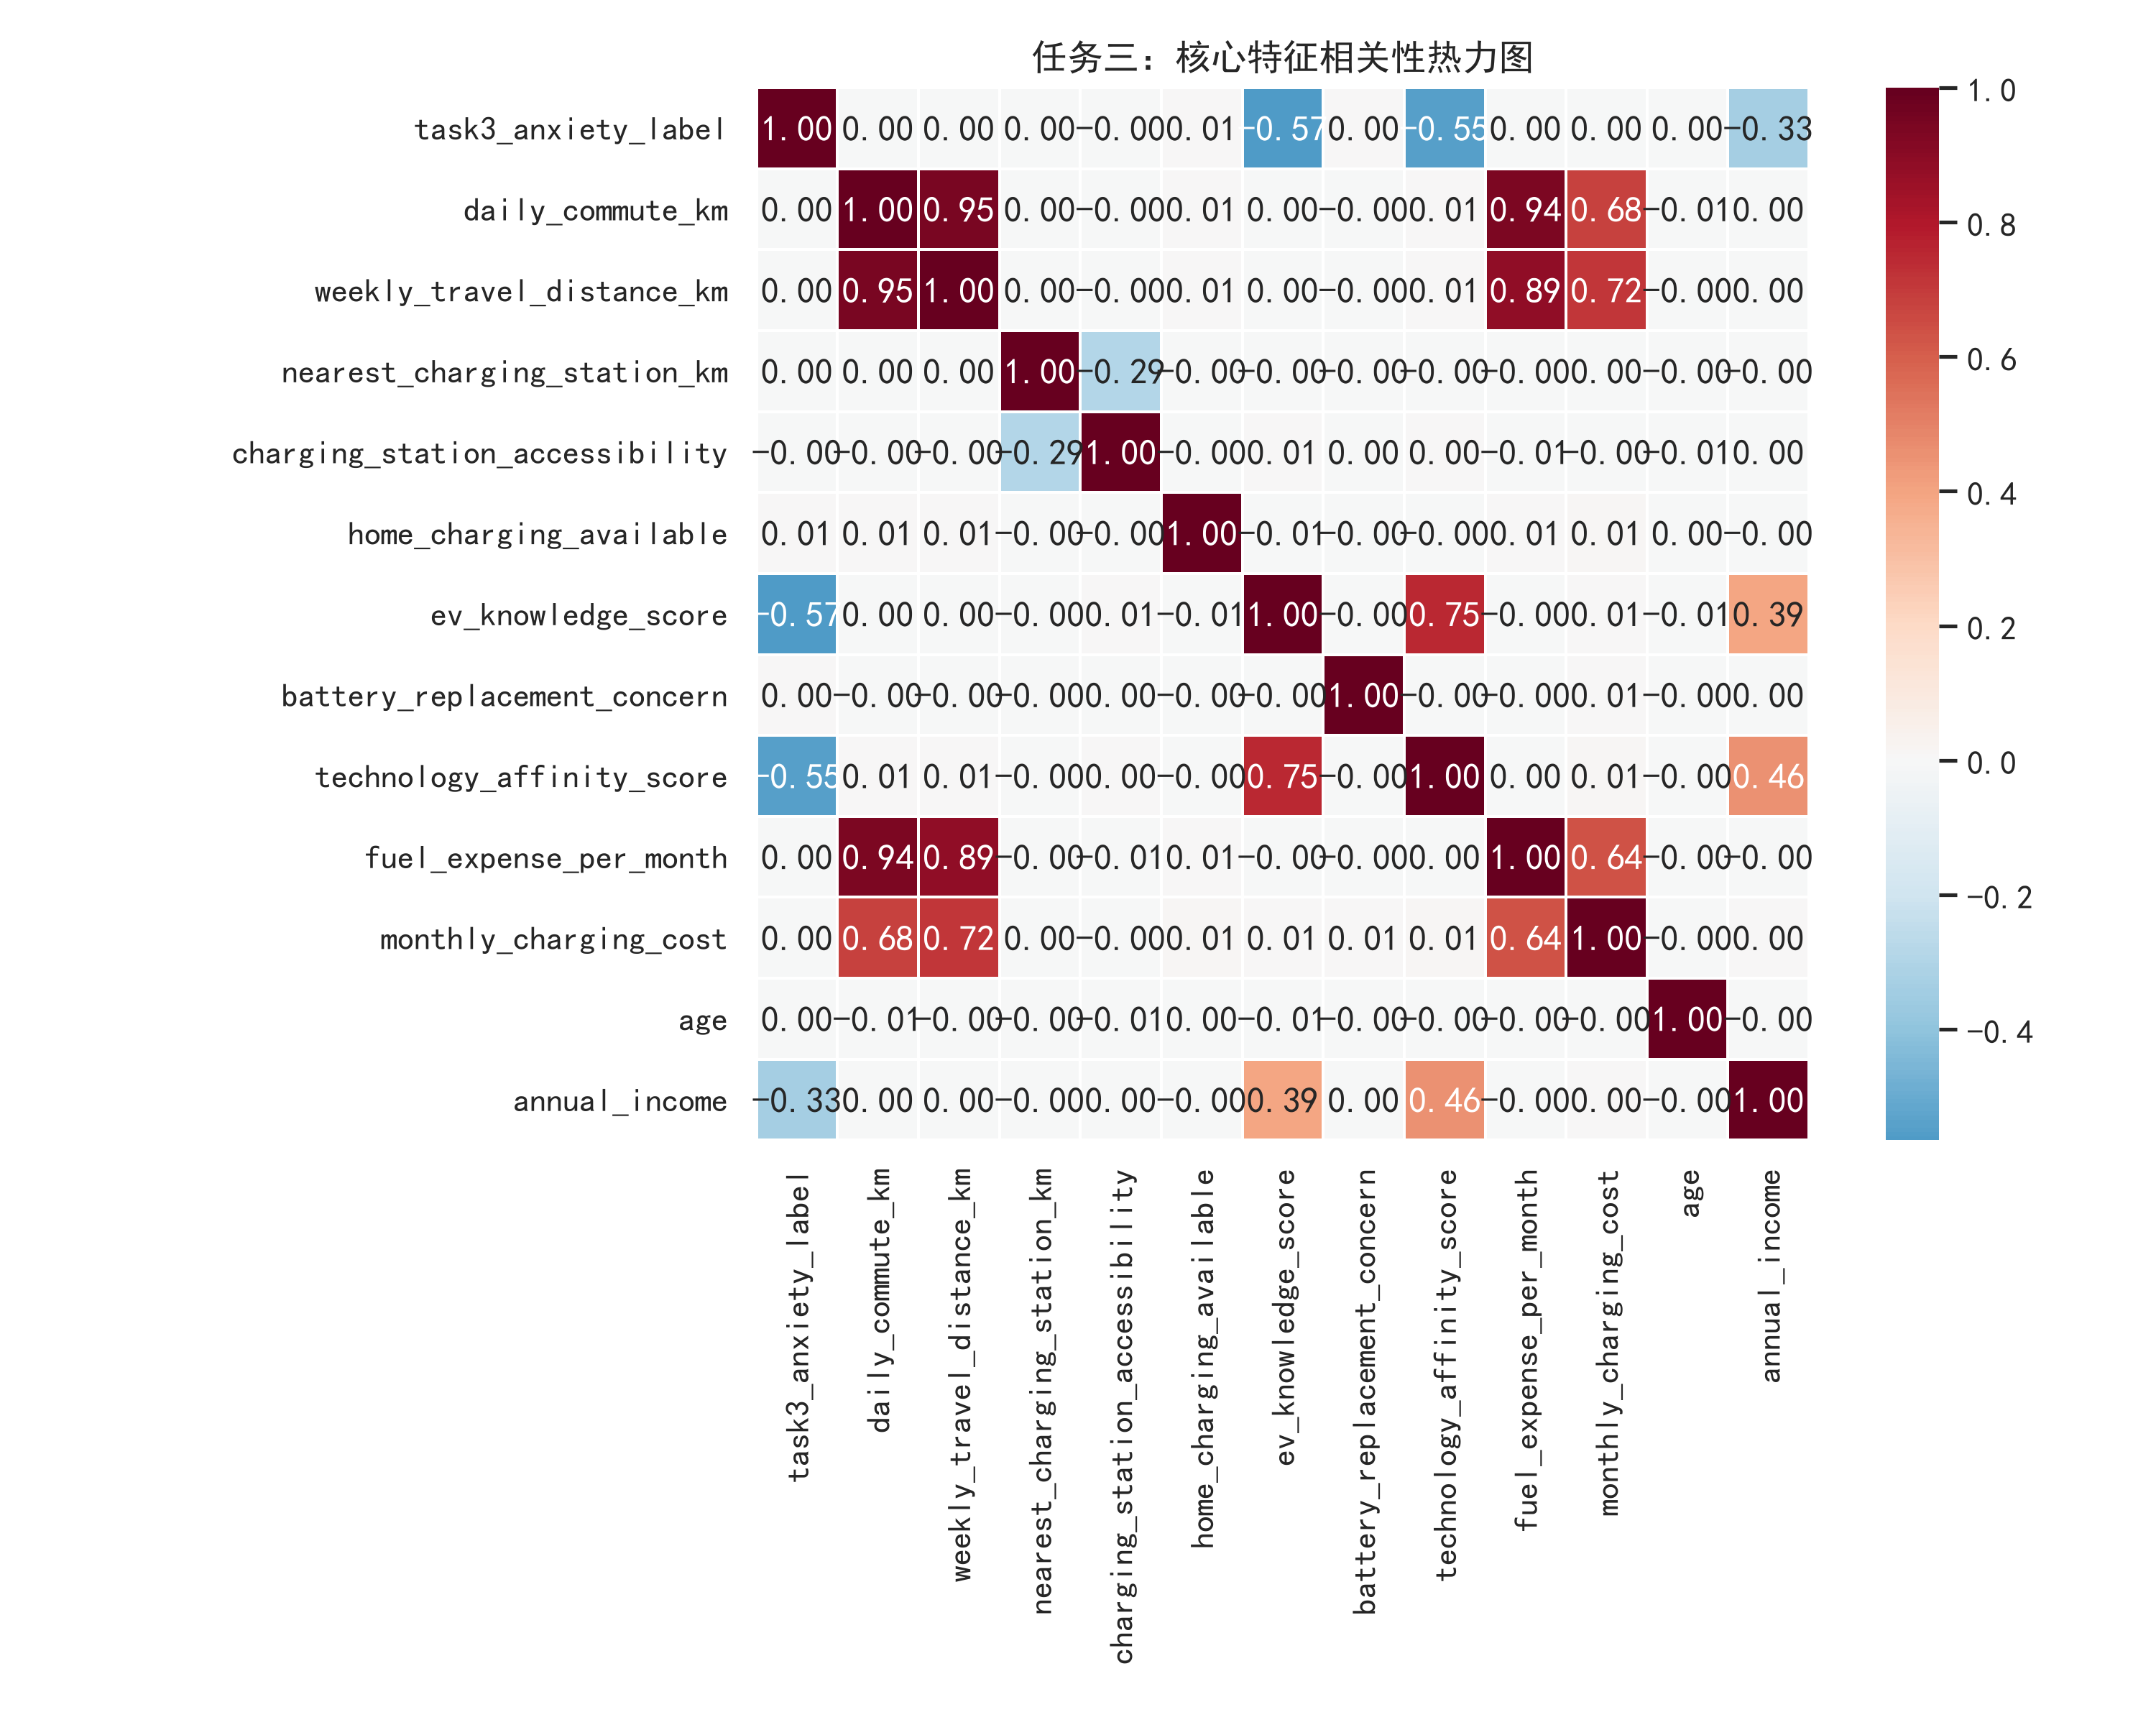
\includegraphics[width=0.85\textwidth]{figures/task3_correlation_heatmap.png}
\caption{任务三核心特征相关性热力图}
\label{fig:t3_corr}
\end{figure}

\subsection{特征工程}

基于上述"认知主导，硬件加成交互"的模式发现，我们为任务三构造了7个业务交互特征（表\ref{tab:t3_features}）。high\_mileage\_low\_convenience依赖训练集分位数阈值，通过fit=True/False接口管理。

\begin{table}[H]
\centering
\caption{任务三业务交互特征}
\label{tab:t3_features}
\begin{tabular}{ccp{4cm}}
\toprule
\textbf{特征} & \textbf{计算公式} & \textbf{业务含义} \\
\midrule
extra\_travel\_intensity & $\text{weekly\_km} - 5 \cdot \text{daily\_km}$ & 额外出行强度 \\
daily\_travel\_approx & $\text{weekly\_km} / 7$ & 日均出行近似 \\
charging\_difficulty & $\dfrac{\text{nearest\_station}}{\text{charge\_access} + 1}$ & 充电困难度 \\
knowledge\_buffer & $\text{ev\_know} - \text{battery\_concern}$ & 知识缓冲量 \\
high\_mileage\_low\_convenience & $\mathbf{1}[\text{weekly\_km} > Q_{75}] \land \mathbf{1}[\text{access} < Q_{25}]$ & 高里程低便利标志 \\
home\_charging\_buffer & $\text{home\_charging} \times \text{daily\_km}$ & 家充缓冲交互 \\
long\_distance\_ratio & $\dfrac{\text{weekly\_km}}{7 \cdot \text{daily\_km} + \varepsilon}$ & 长途占比 \\
\bottomrule
\end{tabular}
\end{table}

\subsection{Main与Ablation消融设计}

\textbf{Main方案（主方案）}：排除ev\_adoption\_likelihood，仅使用可观测特征。采用三阶段递进式调参，超参数搜索范围：depth $\in$ [4,8]，learning\_rate $\in$ [0.02,0.1]，iterations $\in$ [500,1800]，l2\_leaf\_reg $\in$ [3,15]，random\_strength $\in$ [0,2]。loss\_function=Logloss，eval\_metric=Logloss。Main方案共搜索8组参数（40次CV训练）。

\textbf{Ablation方案（消融对照）}：加入ev\_adoption\_likelihood作为分类特征，纯粹用来衡量"若采用意愿已知，焦虑识别能提升多少"。Ablation方案搜索3组参数（15次CV训练）。消融结果仅作参照，不作为可部署方案——采用意愿很可能是焦虑的下游结果，真实预测流程中根本拿不到这个变量。

\subsection{实验结果}

\subsubsection{交叉验证阶段}

Main方案8组参数的5折CV结果如表\ref{tab:t3_cv_main}所示。所有参数组的OOF阈值准确率高度集中（0.86018 -- 0.86077，极差仅0.00059），折间标准差在0.0014 -- 0.0024之间。最佳参数为：depth=8，learning\_rate=0.02，iterations=354，l2\_leaf\_reg=10.0，random\_strength=0.5，OOF阈值准确率=0.86077，OOF AUC=0.90676。

\begin{table}[H]
\centering
\caption{任务三 Main方案 CV阶段结果}
\label{tab:t3_cv_main}
\begin{tabular}{cccccccc}
\toprule
\textbf{Trial} & \textbf{depth} & \textbf{lr} & \textbf{iter} & \textbf{l2} & \textbf{rs} & \textbf{CV ACC} & \textbf{OOF AUC} \\
\midrule
1 & 8 & 0.02 & 500 & 10.0 & 0.5 & 0.86052 & 0.90676 \\
2 & 6 & 0.02 & 800 & 10.0 & 0.5 & 0.86025 & 0.90659 \\
3 & 8 & 0.07 & 1500 & 15.0 & 1.5 & 0.86025 & 0.90589 \\
4 & 4 & 0.10 & 1500 & 3.0 & 0.5 & 0.85992 & 0.90684 \\
5 & 4 & 0.10 & 1500 & 15.0 & 0.5 & 0.86018 & 0.90645 \\
6 & 7 & 0.07 & 1500 & 3.0 & 1.0 & 0.85965 & 0.90630 \\
7 & 7 & 0.10 & 1500 & 7.0 & 1.0 & 0.85967 & 0.90575 \\
8 & 5 & 0.02 & 800 & 3.0 & 0.5 & 0.86050 & 0.90643 \\
\bottomrule
\end{tabular}
\end{table}

一个让人相当放心的现象：所有参数组性能高度集中。这意味着里程焦虑的特征信号确实够强——不同合理参数均能收敛到几乎相同的预测能力。跟任务二中所有参数全部同分的"零信号"模式相比，完全是两个世界。

\subsubsection{验证集方案对比}

在10,000条独立验证集上，各方案的准确率对比如表\ref{tab:t3_results}所示。

\begin{table}[H]
\centering
\caption{任务三验证集方案对比}
\label{tab:t3_results}
\begin{tabular}{lccccc}
\toprule
\textbf{方案} & \textbf{ACC} & \textbf{AUC} & \textbf{Macro F1} & \textbf{Balanced ACC} & \textbf{说明} \\
\midrule
多数类基线 & 0.5079 & 0.5000 & -- & 0.5000 & 全预测为0 \\
LR (无权重) & 0.8311 & -- & 0.8306 & 0.8304 & 可解释性基线 \\
CatBoost 默认 (+业务特征) & 0.8545 & 0.9045 & 0.8541 & 0.8539 & 127轮早停 \\
\textbf{Main 调参（最终）} & \textbf{0.8550} & \textbf{0.9042} & \textbf{0.8546} & \textbf{0.8544} & \textbf{可部署方案} \\
Ablation 调参 & 0.8563 & 0.9145 & 0.8559 & 0.8557 & 仅作对照 \\
\bottomrule
\end{tabular}
\end{table}

Main方案调参后ACC（0.8550）较CatBoost默认（0.8545）仅提升0.05个百分点，这和CV阶段"所有参数性能高度集中"的发现是一致的。Ablation方案加入ev\_adoption\_likelihood后ACC为0.8563，较Main提升0.13个百分点，AUC提升约0.010。

\subsubsection{Main vs Ablation 因果分析}

Ablation虽然在本地实验中跑出了更高的准确率，但这里有个方向性问题。根据赛题的因果关系：高里程焦虑$\to$低采用意愿——焦虑是原因，采用意愿是结果。如果把采用意愿作为输入特征塞进模型，就等于用"结果"来预测"原因"。这是在制造因果倒置。所以我们最终部署选择Main方案（不含ev\_adoption\_likelihood），消融差异如实在论文中报告。

\subsubsection{混淆矩阵}

Main调参模型的验证集混淆矩阵如表\ref{tab:t3_conf}所示。一个值得注意的不对称：高焦虑类误判率（18.2\%）大约是低焦虑类（10.9\%）的1.7倍——高焦虑群体的特征分布更分散，模型更难抓牢。

\begin{table}[H]
\centering
\caption{任务三 Main调参模型混淆矩阵（验证集10,000样本）}
\label{tab:t3_conf}
\begin{tabular}{ccccc}
\toprule
\textbf{真实 $\backslash$ 预测} & \textbf{0（低焦虑）} & \textbf{1（高焦虑）} & \textbf{样本数} & \textbf{误判率} \\
\midrule
0（低焦虑） & 4,525 & 554 & 5,079 & 10.9\% \\
1（高焦虑） & 896 & 4,025 & 4,921 & 18.2\% \\
\bottomrule
\end{tabular}
\end{table}

\subsubsection{特征重要性排名}

Main调参模型特征重要性Top 15如表\ref{tab:t3_import}所示。environmental\_awareness\_score（53.53）和technology\_affinity\_score（31.36）两个变量就占了约85\%的特征重要性——也就是说，两个变量几乎框定了里程焦虑的全部可预测差异。业务交互特征long\_distance\_ratio（第7）、knowledge\_buffer（第12）、charging\_difficulty（第14）均挤入了Top 15的中后段。经济/人口变量的重要性远低于认知变量。里程焦虑说到底是心理/认知现象，特征排名把这一点写得明明白白。

\begin{table}[H]
\centering
\caption{任务三 Main调参模型特征重要性Top 15}
\label{tab:t3_import}
\begin{tabular}{clc}
\toprule
\textbf{排名} & \textbf{特征} & \textbf{重要性} \\
\midrule
1 & environmental\_awareness\_score & 53.53 \\
2 & technology\_affinity\_score & 31.36 \\
3 & annual\_income & 1.43 \\
4 & ln\_income & 1.39 \\
5 & ev\_knowledge\_score & 1.01 \\
6 & government\_incentive\_awareness & 0.94 \\
7 & long\_distance\_ratio $\blacklozenge$ & 0.70 \\
8 & nearest\_charging\_station\_km & 0.63 \\
9 & age & 0.63 \\
10 & vehicle\_age\_years & 0.60 \\
11 & charging\_station\_accessibility & 0.59 \\
12 & knowledge\_buffer $\blacklozenge$ & 0.57 \\
13 & battery\_replacement\_concern & 0.54 \\
14 & charging\_difficulty $\blacklozenge$ & 0.53 \\
15 & electricity\_cost\_per\_kwh & 0.47 \\
\bottomrule
\end{tabular}
\end{table}
注：$\blacklozenge$ 标记为本研究构造的业务交互特征。

\subsubsection{边界样本分析}

边界样本分析是本文的一个独到视角。利用原始评分（仅作模型评估后使用，不参与训练）统计各评分段的准确率，结果如表\ref{tab:t3_boundary}所示。

\begin{table}[H]
\centering
\caption{任务三边界样本分析（原始评分逐段准确率）}
\label{tab:t3_boundary}
\begin{tabular}{cccc}
\toprule
\textbf{原始评分} & \textbf{样本数} & \textbf{准确率} & \textbf{错误率} \\
\midrule
2 & 802 & 0.9925 & 0.0075 \\
3 & 1,320 & 0.9955 & 0.0045 \\
4 & 1,916 & 0.8638 & 0.1362 \\
\textbf{5} & \textbf{1,751} & \textbf{0.6225} & \textbf{0.3775} \\
\textbf{6} & \textbf{1,506} & \textbf{0.6700} & \textbf{0.3300} \\
7 & 969 & 0.9969 & 0.0031 \\
8 & 941 & 0.9979 & 0.0021 \\
9 & 508 & 0.9980 & 0.0020 \\
10 & 287 & 1.0000 & 0.0000 \\
\bottomrule
\end{tabular}
\end{table}

评分距阈值越远，准确率越高——一条清晰的\textbf{V形错误曲线}，谷底恰好扎在评分5（37.75\%错误率）和6（33.00\%错误率）。这条曲线有三层含义：

\begin{enumerate}[itemsep=0pt]
\item \textbf{模型学到了真正的信号}。极端评分近乎完美的准确率排除了"模型在随机猜测"的嫌疑。如果模型没有真正学会焦虑预测的特征模式，所有评分段准确率应该逼近基线（$\approx$51\%），而不是呈现这样有规律的V形曲线。
\item \textbf{边界样本的固有模糊性}。评分5和6的样本占了验证集的32.6\%。对于这些样本，二分标签天然带有问卷评分的主观噪声——一个评分5.0的用户和一个5.1的用户，真实焦虑程度可能毫无差别，标签却恰好被切在了两边。模型的边界混淆反映的是标签二值化在阈值处的不连续性，不是模型能力不足。
\item \textbf{与任务一的对比}。任务一Low/Medium/High之间的误判也呈现对称模式，但任务三的V形曲线尖锐得多——只需跨过约1个评分单位的距离（评分5$\to$7），准确率就从62\%飙升至99.7\%。这暗示range\_anxiety\_score与可用特征之间的关系在群体层面高度连续且可学。
\end{enumerate}

\subsection{跨任务特征比较}

任务一中使用了range\_anxiety\_score构造knowledge\_anxiety\_gap特征（排名第1，得分21.68）。任务三禁止触碰range\_anxiety\_score，我们构造了knowledge\_buffer（ev\_knowledge\_score减去battery\_replacement\_concern）作为替代。两者在结构上类似但经验证无泄漏：battery\_replacement\_concern与range\_anxiety\_score的Pearson相关系数为0.63（中度相关，非函数关系，$R^2=0.40$），仍有约60\%的方差独立。这个替代是干净可用的。
